\documentclass{article}
\usepackage{ebgaramond-maths}
\usepackage[T1]{fontenc}

%==Math & Physics Packages==
\usepackage{amsmath, amsthm, amsfonts, amssymb, physics, cancel, nicefrac, setspace}
\newcommand\arrows[3]{
        \begin{matrix}[c]
        \ifx\relax#1\relax\else \xrightarrow{#1}\fi\\
        \ifx\relax#2\relax\else \xrightarrow{#2}\fi\\
        \ifx\relax#3\relax\else \xrightarrow{#3}\fi
        \end{matrix}
}
\newcommand\aug{\fboxsep=-\fboxrule\!\!\!\fbox{\strut}\!\!\!}
\allowdisplaybreaks

%==Image-related Packages==
\usepackage{dirtree}
\usepackage{graphicx, tikz, pgfplots, xcolor, fourier-orns}
\usetikzlibrary{arrows.meta}
\pgfplotsset{compat=1.18}

%==Colour Palette==
\definecolor{merah}{HTML}{F4564E}
\definecolor{merahtua}{HTML}{89313E}
\definecolor{biru}{HTML}{60BBE5}
\definecolor{birutua}{HTML}{412F66}
\definecolor{hijau}{HTML}{59CC78}
\definecolor{hijautua}{HTML}{366D5B}
\definecolor{kuning}{HTML}{FFD56B}
\definecolor{jingga}{HTML}{FBA15F}
\definecolor{ungu}{HTML}{8C5FBF}
\definecolor{lavender}{HTML}{CBA5E8}
\definecolor{merjamb}{HTML}{FFB6E0}

%==Formatting Packages==

\usepackage{float}
\usepackage{caption}
\usepackage{tocbasic}
\renewcommand*{\tableofcontents}{\listoftoc[\contentsname]{toc}}
\renewcommand*{\listoffigures}{\listoftoc[\listfigurename]{lof}}
\renewcommand*{\listoftables}{\listoftoc[\listtablename]{lot}}
\setuptoc{lof}{leveldown,totoc}
\setuptoc{lot}{leveldown,totoc}
\usepackage{multicol, indentfirst, fontsize}
%\usepackage[toc]{multitoc}


\renewcommand*\contentsname{Daftar Isi}
\renewcommand{\figurename}{Gambar}
\captionsetup[table]{name=Tabel}
%\renewcommand*{\multicolumntoc}{2}
\setlength{\columnseprule}{1.5pt}

\usepackage{tcolorbox}
\tcbuselibrary{skins,breakable,theorems}
\usepackage{changepage}

\newcounter{hitung}
\setcounter{hitung}{\thesection}

\makeatletter
% Proof
\def\tcb@theo@widetitle#1#2#3{\hbox to \textwidth{\textsc{\large#1}\normalsize\space#3\hfil(#2)}}
\tcbset{
	theorem style/theorem wide name and number/.code={ \let\tcb@theo@title=\tcb@theo@widetitle},
	proofbox/.style={skin=enhancedmiddle,breakable,parbox=false,boxrule=0mm,
		check odd page, toggle left and right, colframe=black!20!white!92!hijau,
		leftrule=8pt, rightrule=0mm, boxsep=0mm,arc=0mm, outer arc=0mm,
		left=3mm,right=3mm,top=0mm,bottom=0mm, toptitle=0mm,
		bottomtitle=0mm,colback=gray!3!white!98!biru, before skip=8pt, after skip=8pt,
		before={\par\vskip-2pt},after={\par\smallbreak},
	},
}
\newtcolorbox{ProofBox}{proofbox}
\makeatother

\let\realproof\proof
\let\realendproof\endproof
\newenvironment{soln}[1][Solusi.]{\ProofBox\strut\textsc{#1}\space}{\endProofBox}

% Definition
\newtcbtheorem[use counter=hitung, number within=section]{dfn}{Definisi}
{theorem style=theorem wide name and number,breakable,enhanced,arc=0mm,outer arc=0mm,
	boxrule=0pt,toprule=1pt,leftrule=0pt,bottomrule=1pt, rightrule=0pt,left=0.2cm,right=0.2cm,
	titlerule=0.5em,toptitle=0.1cm,bottomtitle=-0.1cm,top=0.2cm,
	colframe=white!10!hijau,colback=white!90!hijau,coltitle=white,
	coltext=black!45!hijau, title style={white!10!hijau}, before skip=8pt, after skip=8pt,
	fonttitle=\bfseries,fontupper=\normalsize}{dfn}

% Theorem
\newtcbtheorem[use counter=hitung, number within=section]{thm}{Teorema}
{theorem style=theorem wide name and number,breakable,enhanced,arc=0mm,outer arc=0mm,
	boxrule=0pt,toprule=1pt,leftrule=0pt,bottomrule=1pt, rightrule=0pt,left=0.2cm,right=0.2cm,
	titlerule=0.5em,toptitle=0.1cm,bottomtitle=-0.1cm,top=0.2cm,
	colframe=white!10!merah,colback=white!75!pink,coltitle=white, coltext=merahtua!80!merah,
	title style={white!10!merah}, before skip=8pt, after skip=8pt,
	fonttitle=\bfseries,fontupper=\normalsize}{thm}


% Example
\newtcolorbox[use counter=hitung, number within=section]{cth}[1][]{breakable,
	colframe=black!40!gray, coltitle=white, colback=white, coltext=black!80!gray, colbacktitle=black!40!gray, enhanced, fonttitle=\bfseries,fontupper=\normalsize, attach boxed title to top left={yshift=-2mm}, before skip=8pt, after skip=8pt,
	title=Contoh~\thetcbcounter \ \ #1}

% Catatan
\newtcbtheorem[use counter=hitung, number within=section]{rmr}{Catatan}
{theorem style=theorem wide name and number,breakable,enhanced,arc=0mm,outer arc=0mm,
	boxrule=0pt,toprule=1pt,leftrule=0pt,bottomrule=1pt, rightrule=0pt,left=0.2cm,right=0.2cm,
	titlerule=0.5em,toptitle=0.1cm,bottomtitle=-0.1cm,top=0.2cm,
	colframe=white!10!biru,colback=white!90!biru,coltitle=white, coltext=birutua!80!gray,
	title style={white!10!biru}, before skip=8pt, after skip=8pt,
	fonttitle=\bfseries,fontupper=\normalsize}{rmr}


%==Layouting Packages==
\usepackage{titlesec, fancyvrb, listings, upquote}
\setlength{\headheight}{14.39996pt}
\lstdefinestyle{default}{
	commentstyle=\color{black!20!hijau},
	keywordstyle=\color{purple!100!purple},
	numberstyle=\scriptsize\color{black},
	stringstyle=\color{black!30!biru},
	basicstyle=\fontfamily{IBMPlexMono-TLF}\small,
	breakatwhitespace=false,         
	breaklines=true,                 
	captionpos=b,                    
	keepspaces=true,                 
	numbers=left,                    
	frame=single,
	showspaces=false,                
	showstringspaces=false,
	showtabs=false,                  
	tabsize=2,
}
\lstdefinestyle{noangka}{
	numbers=none,
}
\lstset{style=default}
\titleformat{\paragraph}[runin]{\normalfont\bfseries}{\theparagraph}{1em}{}
\newcounter{subsubsubsection}  
\setcounter{subsubsubsection}{0}  

\newcommand{\subsubsubsection}[1]{%
  \refstepcounter{subsubsubsection}  
  \paragraph*{\thesubsubsection.\arabic{subsubsubsection}\quad #1} 
}

\newcommand{\fpb}[2]{\mathrm{FPB}(#1, #2)}
\newcommand{\kpk}[2]{\mathrm{KPK}(#1, #2)}

%Reference and Bibliography Packages==
\renewcommand{\listtablename}{Daftar Tabel}
\renewcommand{\listfigurename}{Daftar Gambar}
\usepackage{hyperref}
\hypersetup{
	colorlinks=true,
	linkcolor={merah!40!black},
	citecolor={biru!20!black},
	urlcolor={black!40!biru!70!blue}
}

\numberwithin{equation}{section}

% Silakan lihat dokumentasi package biblatex
% untuk format sitasi yang diperlukan
\usepackage[backend=biber]{biblatex}
\makeatletter
\def\@biblabel#1{}
\makeatother

\renewcommand{\mod}{\mathrm{mod} \ }


%Titling
\usepackage{etoolbox}
\makeatletter
\providecommand{\institute}[1]{% add institute to \maketitle
  \apptocmd{\@author}{\end{tabular}
    \par
    \begin{tabular}[t]{c}
    #1}{}{}
}
\makeatother

\newcommand{\garis} [3] []{
	\begin{center}
		\begin{tikzpicture}
			\draw[#2-#3, ultra thick, #1] (0,0) to (1\linewidth,0);
		\end{tikzpicture}
	\end{center}
}

\renewcommand\today{$\number\day$\ %
	\ifcase\month \or Januari%
	\or Februari%
	\or Maret%
	\or April%
	\or Mei%
	\or Juni%
	\or Juli%
	\or Agustus%
	\or September%
	\or Oktober%
	\or November%
	\or Desember\fi\ $\number\year$}%

 %%%%%%%%%%%%%%%%%%%%%
 %%%%%%% JUDUL %%%%%%%
 %%%%%%%%%%%%%%%%%%%%%
 \title{
\textbf{Laporan Tugas Besar 1} 
\\ IF$2123$ Aljabar Linear dan Geometri \\[5em]
}

\author{
{\centering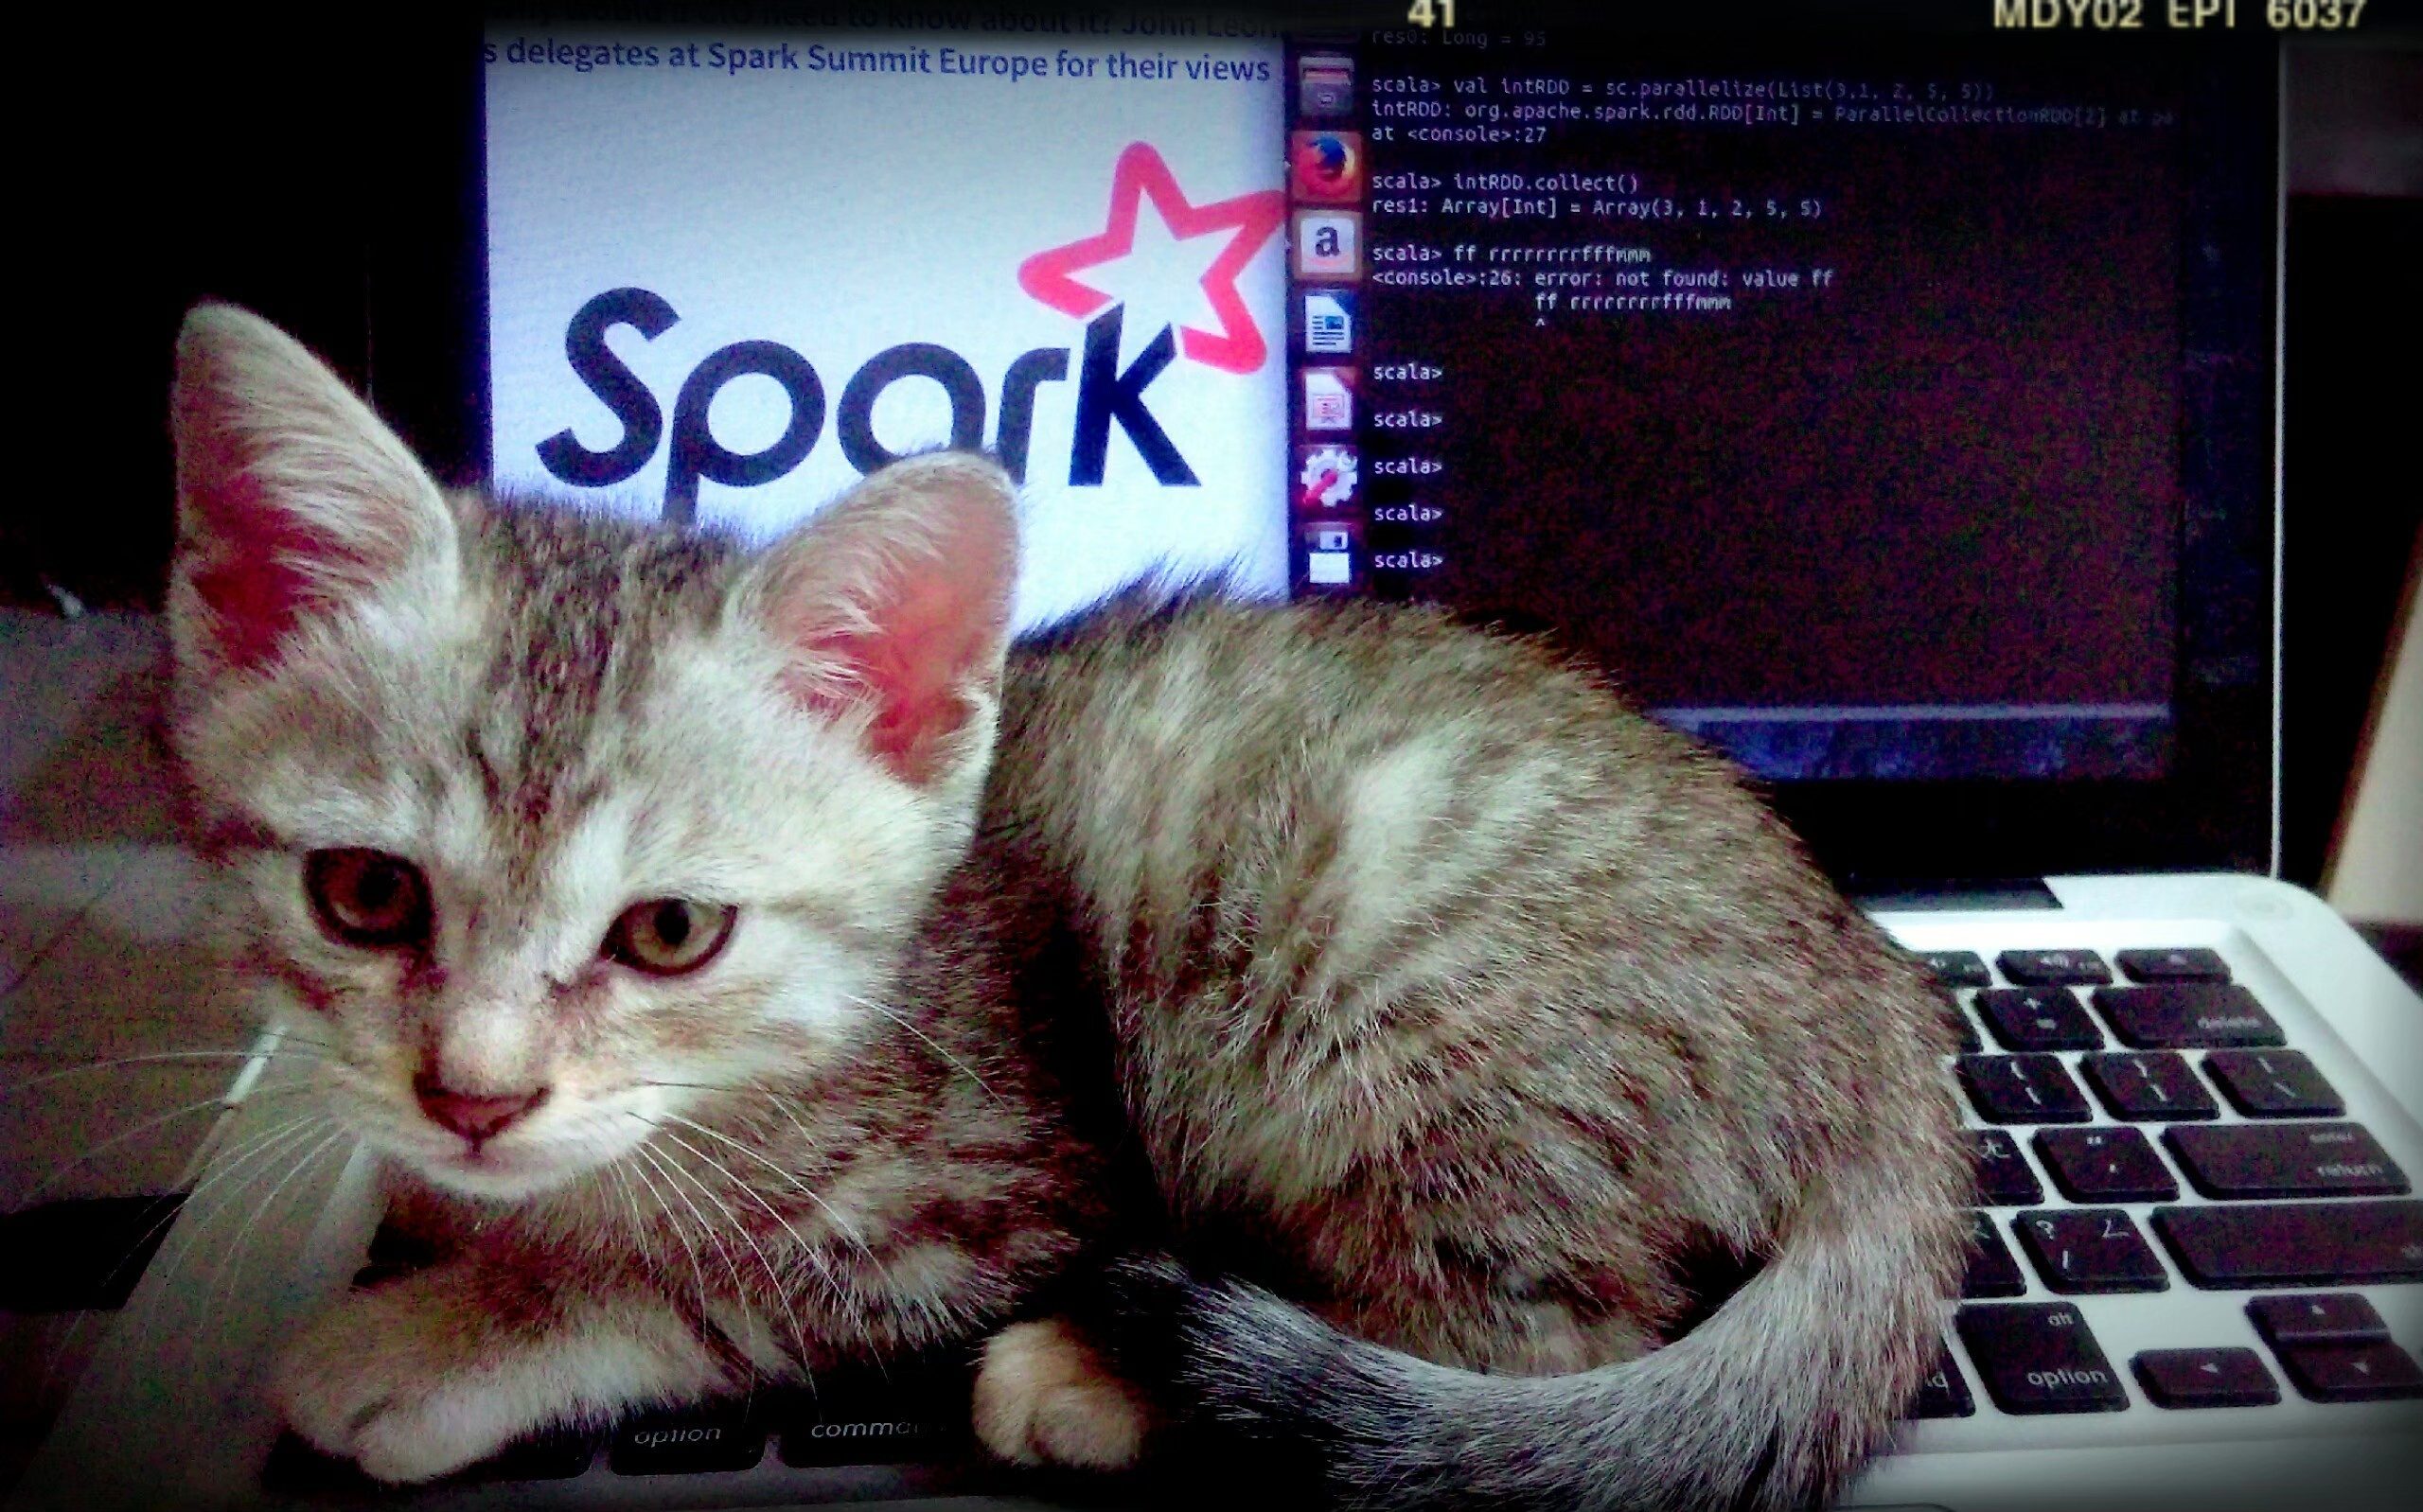
\includegraphics[scale=0.1]{cat.jpg} } \\[2.5em]
$\begin{array}{ll}
    \text{Muhammad Luqman Hakim}           & 13523044 \\ 
    \text{Zulfaqqar Nayaka Athadiansyah}   & 13523094 \\ 
    \text{Farrel Athalla Putra}            & 13523118 \\[5em]
\end{array}$
    } 


\date{\Large\textbf{Program Studi Teknik Informatika \\
Sekolah Teknik Elektro dan Informatika \\
Institut Teknologi Bandung \\
2024}}